\documentclass{article}
\usepackage[utf8]{inputenc}
\usepackage[margin=1.2in]{geometry}
\usepackage{amsmath,amssymb}
\usepackage{graphicx}
\usepackage{esvect}
\usepackage{fancyhdr}
\usepackage{amsthm}
\usepackage{tikz}
\usepackage{color}   %May be necessary if you want to colour links
\usepackage{hyperref}
\usepackage{lastpage}

\hypersetup{
    colorlinks=true, %set true if you want colored links
    linktoc=all,     %set to all if you want both sections and subsections linked
    linkcolor=blue,  %choose some color if you want links to stand out
}
% \pagestyle{plain}
% \pagestyle{fancy}
% % \fancyhf{}
% \cfoot{}
% \fancyfoot[R]{Page \thepage\ of }

\theoremstyle{plain}
\newtheorem{theorem}{Theorem}
\newtheorem{proposition}{Proposition}


\theoremstyle{definition}
\newtheorem{definition}{Definition}
\newtheorem{example}{Example}

\theoremstyle{remark}
\newtheorem{rem}{Remark}



% Custom Commands 
\newcommand{\R}{\mathbb{R}}


\title{Differential Geometry of Surfaces}
\author{Pankaj Ghodla }
% \date{January 2021}

\begin{document}
\maketitle
\tableofcontents

\newpage


\section{Introduction}
In this section, we will introduce some of the basic definition of curves and surfaces.
\subsection{Curves}
Intuitively, A curves can be thought as the trace of a moving particle in the space. Mathematical, a curves is defined to be the image of a function, \( \gamma: U \rightarrow \R^n \), where U \( \subset \R \)..

\begin{definition}[Parametrised curve]
    A \textbf{parametrised curve} in \( \R^n \) is a smooth function \( \gamma: U \rightarrow \R^n \), where U \( \subset \R \).
\end{definition}
Throughout, this report we will assume that smoothness mean \( \text{C}^\infty \), i.e. the function is differentiable infinitely many times.

\begin{definition}[Regular curve]
    Let \( \gamma: U \rightarrow \R^n \) be a curve. It is called regular if its derivative is non-vanishing, i.e. \( \left\lVert  \gamma^\prime(t) \right\rVert \neq 0 \), \( \forall \in U \).
\end{definition}

There are many different ways to parametrise a curve, e.g. \( \gamma(t) = (t, t^2)\) and \( \tilde{\gamma}(t) = (t^2, t^4)\). However, only one of these curve is regular, which is \( \gamma(t) \). Moreover, there are many different ways to parametrise a curves such that all the parametrisations are regular.

\begin{definition}[Unit speed curve]
    Let \( \gamma: U \rightarrow \R^n \) be a curve. It is called unit-speed, if \( \left\lVert  \gamma^\prime(t) \right\rVert = 1 \), \( \forall \in U \).
\end{definition}
We will see later on that a lot of the formulas and results relating to curves take on a much simpler form when the curve is unit-speed, e.g. curvature of a unit-speed curve, see definition \ref{definition: Curvature of a curve}, is just the norm of it's second derivative.

\begin{proposition}
    A parametrised curve is unit-speed if and only if it is regular.
\end{proposition}
{\color{red} proof ??}

{\color{red} Explain in more detail why curvature is defined in the following manner: }
\begin{definition}[Curvature of a curve] \label{definition: Curvature of a curve}
    Let \( \gamma: U \rightarrow \R^n \) be a unit-speed curve. The curvature at point \( \gamma(t) \) is defined as \[ \kappa(t) = \left\lVert \gamma^{\prime\prime} \right\rVert  \]
\end{definition}

These are all the definitions and results about curves that we need to know to understand this report.
\subsection{Surfaces}
Intuitively, a surface is a subset of \( \R^3 \) that looks like a \( \R^2 \)  in the neighbourhood of any given point, e.g. the surface of the Earth is spherical; however, it appear to be a flat plane(\( \R^2 \)) to an observer on the surface.

\begin{definition}[Diffeomorphism]
    if \( f: U \rightarrow W \) is continuous, bijective, and smooth, and if its inverse maps \( f^{-1}: W \rightarrow U\) is also continuous and smooth, then f is called a diffeomorphism and \(U\) and \(W\) are called diffeomorphic.
\end{definition}

\begin{definition}[Regular Surface]
    A subset of \( \R^3 \) is a regular surface, if every point P \( \in S \), there exists a open set \( U \text{ in } \R^2\) and an open set \( W \text{ in } \R^3\) containing P such that \( S \cap W\) is diffeomorphic to \(U\).
\end{definition}
Therefore, a surface is collection of diffeomorphisms, \( \sigma: U \rightarrow S \cap W \), which we call regular surface patches.

\begin{definition}[Reparametrisation of surface patches]
    Let \( \sigma: U \rightarrow S\) and \( \tilde{\sigma}: \tilde{U} \rightarrow S\) be surface patches for a surface S, then \( \tilde{\sigma} \) is called a reparametrisation of \( \sigma \) if there exists a map, \( \Phi: \tilde{U} \rightarrow U \), which is smooth and bijective with smooth inverse, \( \Phi^{-1}: U \rightarrow \tilde{U} \).
\end{definition}

\begin{definition}[Tangent space]
    Let \(S\) be a regular surface. The \textbf{tangent plane} to \(S\) at the point \( p \in S\) is the set of all initial velocity vectors of regular curves in \(S\) with initial position \(p\), i.e \[ T_pS = \{ \gamma^\prime(0) | \gamma \text{ is a regular curve in S with }\gamma(0) = p\} \]
\end{definition}

These are all the definitions about surfaces that we need to understand this report.

\section{First Fundamental Form}
In this section, we will define one of the most important object that lets us compute lengths, angles and areas on surface. It is called the \textbf{first fundamental form}.

{\color{red} Change this definition}

\begin{definition}[The fundamental form]
    The \textbf{first fundamental form} is the restriction of the inner product of the ambient space(\(\R^3\)) to the tangent space(\( T_pS\)) at point \( p \in S\). The first fundamental form is denoted by \( \mathbf{I} \), \[ \mathbf{I}(x,y) = \left\langle x,y\right\rangle  \], where \( x,y \in T_pS\).
\end{definition}

\subsection{The first fundamental form in local coordinates}
We'll now discuss the classical notation for expressing the first fundamental form in local coordinates. Suppose \( \sigma(u,v): U \rightarrow S\) is a surface patch and \( x,y \in T_pS \), where \(T_pS\) is the tangent plane at point \(p\) on \(S\). Let \( \sigma(u_0, v_0) = p \) and \( f_u = \sigma_u \mid_{u_0} \) and \( f_u = \sigma_v \mid_{v_0} \). Then, we can write \(x =  f_u a + f_v b\) and \( y =  f_u c + f_v d\). This implies the following:
\begin{align}
    \begin{split}
        \mathbf{I}(x,y) & = \mathbf{I}( f_u a + f_v b,  f_u c + f_v d) \\
        & = \left\langle f_u a + f_v b,  f_u c + f_v d \right\rangle \\
        & = ac\left\langle  f_u  +,  f_u  \right\rangle + (ad+bc)\left\langle  f_u  , f_v  \right\rangle + bd \left\langle f_v , f_v  \right\rangle \\
        & = ac E + (ad+bc)F + bd G
    \end{split}
\end{align}

% Suppose \( \sigma: U \rightarrow S\) is a surface patch and \(\gamma(t): X \rightarrow S\) is a curve on the surface patch of S, defined as \( \gamma(t) = \sigma(u(t),v(t))\). Let \( \gamma(t_0) = p \in S \), then using the chain rule we know that \( \gamma^\prime = \sigma_u u^\prime +  \sigma_v v^\prime\).
% We may then compute:
% \begin{align}
%     \left\langle \gamma^\prime, \gamma^\prime\right\rangle
%      & = \left\langle \sigma_u u^\prime +  \sigma_v v^\prime ,  \sigma_u u^\prime,  \sigma_v v^\prime\right\rangle \nonumber                                                                                                                                                                                                                         \\
%      & = \left\langle \sigma_u u^\prime, \sigma_u u^\prime\right\rangle (u^\prime)^2 + \left\langle \sigma_u u^\prime, \sigma_v v^\prime\right\rangle (u^\prime v^\prime) + \left\langle \sigma_v v^\prime, \sigma_u u^\prime\right\rangle v^\prime u^\prime + \left\langle \sigma_v v^\prime, \sigma_v v^\prime\right\rangle (v^\prime)^2 \nonumber \\
%      & = \left\langle \sigma_u u^\prime, \sigma_u u^\prime\right\rangle (u^\prime)^2 + 2\left\langle \sigma_u u^\prime, \sigma_v v^\prime\right\rangle (u^\prime v^\prime) + \left\langle \sigma_v v^\prime, \sigma_v v^\prime\right\rangle (v^\prime)^2 \nonumber                                                                                   \\
%      & = E(u^\prime)^2 + 2F u^\prime v^\prime + G (v^\prime)^2
% \end{align}

where
\begin{align}
    E = \left\lVert f_u \right\rVert ^2, F = \left\lVert f_u f_v\right\rVert ,  G = \left\lVert
    f_v \right\rVert ^2
\end{align}

\begin{definition}[the first fundamental form]
    The first fundamental form in local coordinates(\(u,v\)) is the expression \(\mathcal{F}_1 =  E du^2 + 2F du dv + G dv^2 \).
\end{definition}

Now, a good question to ask would be, how reparametrisation of a surface affects the first fundamental form of the surface in terms of the local coordinates?

\begin{example}
    Let \(S\) be a surface. Suppose \(\tilde{\sigma}: \tilde{U} \rightarrow S \) is a reparametrisation of \(\sigma: U \rightarrow S \), where \(\sigma\) is a surface patch of \(S\) and \( U, \tilde{U} \subset \R^2 \).
    Assume that \( \Phi: \tilde{U} \rightarrow U\) is a smooth map and the following are the first fundamental form of \(\tilde{\sigma}\) and \(\sigma\), respectively:
    \begin{align*}
        \tilde{E} d\tilde{u}^2 + 2\tilde{F} d\tilde{u} d\tilde{v} + G d\tilde{v}^2
        \text{  and  }
        E du^2 + 2F du dv + G dv^2
    \end{align*}
    Then,
\end{example}
\begin{align} \label{eq: reparmetrisation affect on the first fundamental form}
    \begin{pmatrix}
        \tilde{E} & \tilde{F} \\
        \tilde{F} & \tilde{G}
    \end{pmatrix}
    =
    J(\Phi)^t
    \begin{pmatrix}
        E & F \\
        F & G
    \end{pmatrix}
    J(\Phi)
\end{align}

, where \( J(\Phi) \) is the Jacobian of \(\Phi\), i.e.

\begin{align*}
    J(\Phi) =
    \begin{pmatrix}
        \frac{\partial u}{ \partial \tilde{u}} &  & \frac{\partial u}{ \partial \tilde{v}} \\
        \frac{\partial v}{ \partial \tilde{u}} &  & \frac{\partial v}{ \partial \tilde{v}}
    \end{pmatrix}
\end{align*}

\begin{proof}[Proof]
    We know that
    \( \tilde{\sigma} (\tilde{u}, \tilde{v}) = \sigma(\Phi(\tilde{u}, \tilde{v})) = \sigma(u,v)\) and
    \( \tilde{E} = \left\lVert \tilde{\sigma}_{\tilde{u}}\right\rVert^2 \text{ , and } E = \left\lVert \sigma_u \right\rVert^2 \). \\
    Then,
    \begin{align*}
        \tilde{E} & = \left\lVert \tilde{\sigma}_{\tilde{u}}\right\rVert^2                                                                                                                                                         \\
                  & = \left\lVert (\sigma \circ \Phi)_{\tilde{u}}\right\rVert^2                                                                                                                                                    \\
                  & = \left( \sigma_u \frac{\partial u}{ \partial \tilde{u}} + \sigma_v \frac{\partial v}{ \partial \tilde{u}}\right) ^2                                                                                           \\
                  & = \sigma_u^2 \frac{\partial u}{ \partial \tilde{u}}^2 + 2\sigma_u \sigma_v \frac{\partial u}{ \partial \tilde{u}} \frac{\partial v}{ \partial \tilde{u}} + \sigma_v^2 \frac{\partial v}{ \partial \tilde{u}}^2 \\
                  & = E \frac{\partial u}{ \partial \tilde{u}}^2 + 2F \frac{\partial u}{ \partial \tilde{u}} \frac{\partial v}{ \partial \tilde{u}} + G \frac{\partial v}{ \partial \tilde{u}}^2
    \end{align*}
    Similarly,
    \begin{align*}
        \tilde{G} & = \sigma_u^2 \frac{\partial u}{ \partial \tilde{v}}^2 + 2\sigma_u \sigma_v \frac{\partial u}{ \partial \tilde{v}} \frac{\partial v}{ \partial \tilde{v}} + \sigma_v^2 \frac{\partial v}{ \partial \tilde{v}}^2 \\
                  & = E \frac{\partial u}{ \partial \tilde{v}}^2 + 2F \frac{\partial u}{ \partial \tilde{v}} \frac{\partial v}{ \partial \tilde{v}} + G \frac{\partial v}{ \partial \tilde{v}}^2                                   \\
        \tilde{F} & = \sigma_u^2 \frac{\partial u}{ \partial \tilde{u}} \frac{\partial u}{ \partial \tilde{v}} +
        \sigma_u \sigma_v \frac{\partial u}{ \partial \tilde{u}} \frac{\partial v}{ \partial \tilde{v}} +
        \sigma_v \sigma_u \frac{\partial v}{ \partial \tilde{u}} \frac{\partial u}{ \partial \tilde{v}} +
        \sigma_v^2 \frac{\partial v}{ \partial \tilde{u}} \frac{\partial v}{ \partial \tilde{v}}                                                                                                                                   \\
                  & = E \frac{\partial u}{ \partial \tilde{u}} \frac{\partial u}{ \partial \tilde{v}} +
        F \frac{\partial u}{ \partial \tilde{u}} \frac{\partial v}{ \partial \tilde{v}} +
        F \frac{\partial v}{ \partial \tilde{u}} \frac{\partial u}{ \partial \tilde{v}} +
        G \frac{\partial v}{ \partial \tilde{u}} \frac{\partial v}{ \partial \tilde{v}}
    \end{align*}

    Therefore, if we write this in a matrix form we would get equation \ref{eq: reparmetrisation affect on the first fundamental form}.

\end{proof}
\subsection{Length, Angle, and Area}
Now, you may be wondering how do we calculate the lengths, angles and areas on the surface as we claimed before. To calculate the length, let \( \gamma: X \rightarrow S \) be a curve on the surface, where \(X \subset \R \). Then,
\begin{align*}
    l = \int_{t_0}^{t_1} \left\lVert \gamma(t)\right\rVert dt
\end{align*}
\(l\) is the length of the \(\gamma\) from \(t_0\) to \(t_1\), where \( t_0, t_1 \in X\).
To calculate the angle between two tangent vectors, we can use the definition of inner product, i.e. \( \left\langle x, y\right\rangle = cos(\theta) \left\lVert x \right\rVert \left\lVert y \right\rVert  \), where \(\theta\) is the angle between the tangent vectors. Therefore,
\begin{align*}
    \theta = cos^{-1} \left(  \frac{\left\langle x, y\right\rangle }{\left\lVert x \right\rVert \left\lVert y \right\rVert } \right)
\end{align*}
% first we need to represent the inner product on tangent space in terms of the norm of vectors. Let \( x,y \in T_pS\) then,
% \begin{align*}
%     \left\langle x, y\right\rangle = \frac{1}{2}(\left\lVert x\right\rVert^2 + \left\lVert y\right\rVert^2 +\left\lVert x-y \right\rVert  )
% \end{align*}
% Now, we can calculate the angle between two vectors in the tangent plane using the following forma:
% \begin{align*}
%     \left\langle x,y\right\rangle & = \left\lVert x\right\rVert \left\lVert y\right\rVert \text{cos}(\theta)                                                                                                                              \\
%     \therefore \theta             & = \text{cos}^{-1} \left( \frac{\left\langle x,y\right\rangle }{\left\lVert c\right\rVert \left\lVert y\right\rVert } \right)                                                                          \\
%                                   & = \text{cos}^{-1} \left( \frac{\frac{1}{2}(\left\lVert x\right\rVert^2 + \left\lVert y\right\rVert^2 +\left\lVert x-y \right\rVert  ) }{\left\lVert x\right\rVert \left\lVert y\right\rVert } \right)
% \end{align*}
To calculate the area, we first need to represent the norm of the cross product of \( \sigma_u \) and \( \sigma_v \) in terms of the first fundamental form, where \( u \) and \( v\) are local coordinates.
\begin{align*}
    \left\lVert \sigma_u \times \sigma_v \right\rVert & = \sqrt{\left\lvert \sigma_u\right\rvert^2 \left\lvert \sigma_v \right\rvert^2 - \left\langle \sigma_u, \sigma_v \right\rangle } \\
                                                      & = \sqrt{EG - F^2}
\end{align*}

Therefore, the area of the region \( \sigma(U) \), where \( U \subset \R^2 \), is :
\begin{align*}
    Area(U) & = \iint_U \left\lVert \sigma_u \times \sigma_v \right\rVert dA \\
            & = \iint_U \sqrt{EG - F^2} dA
\end{align*}

\section{Second Fundamental Form}
In this section, we will learn about the Gauss map, the intuition behind the second fundamental form, normal curvature, and geodesic curvature. We'll also discuss the mathematical formulas for these concepts.

\begin{definition}[Gauss Map]
    The \textbf{Gauss Map} on a surface \(S\) is just a smooth map defined on the surface \(S\) to \(S^2\), i.e. \( N: S \rightarrow S^2 \), where \( S^2\) is the contour of a unit sphere.
\end{definition}
In other words, the Gauss map is just a unit normal vector field N, where we imagine the output vectors drawn from the origin.\\
For \( p \in S\), consider the derivative \(dN_p: T_pS \rightarrow T_{N(p)}S \). We notice that the domain and codomain of the derivative are the same subspace of \( \R^3\) because \(N(p)\) is normal to the surface \(S\) and \(S^2\).

\begin{definition}[Orientabile]
    A surface is called orientable if we can make a consistent choice of surface normal vector at every point on the surface. In other words, if we can define a Gauss map on the entire surface then it is orientable.
\end{definition}
\begin{definition}[Weingarten Map]
    Let \(S\) be an orientable surface and N be the \textbf{Gauss map} on \(S\). Then, for every point \(p \in S \) the linear transformation
    \begin{align*}
        \mathcal{W}_p = -dN_p: T_pS \rightarrow T_pS
    \end{align*}
    is called the \textbf{Weingarten map} of \(S\) at \(p\).
\end{definition}
The negative sign in the definition of Weingarten map may seen weird at first; however, it will become clear when we talk about the normal curvature. It can be shown that the Weingarten map can be represent as a diagonal matrix with a change in basis; however, we will not prove this here.

\subsection{Normal and Geodesic Curvature}
We'll now discuss about the normal curvature. Intuitively, it measures of how quickly the surface is bending away from the the tangent plane at a point on the surface in a given direction. Mathematical, we define it as follows:

\begin{definition}[Normal Curvature]
    Let \(S\) be an orientable surface, \( p \in S\). Suppose \( \gamma: X \subset \R^2 \rightarrow S\) is a unit speed curve, \( \gamma(0) = p\) and \(\gamma^{\prime}(0) = v\). Then, the normal curvature \(( \kappa_n) = \left\langle y^{\prime \prime}(0), N(p)\right\rangle \).
\end{definition}
We can intuitively see that \(\kappa_n\) measures how fast a curve is curving at point \(p\) away from the tangent plane \(T_pS\), see figure \ref{fig:normal_and_geodesic_curvature}.
It turns out that there is another equivalent definition of the normal curvature. It can be seen by the following calculation:
\begin{align}
    \begin{split}
        & 0 = \left\langle \gamma^{\prime}(t) , N(\gamma(t)) \right\rangle \\
        & \implies \frac{d}{dt} \bigm|_{t=0} 0  = \frac{d}{dt} \bigm|_{t=0} \left\langle \gamma^{\prime}(t) , N(\gamma(t)) \right\rangle 
        = \left\langle \gamma^{\prime \prime}(t), N(p)\right\rangle + \left\langle v, dN_p(v) \right\rangle \\
        & \implies  - \left\langle v, dN_p(v) \right\rangle  = \left\langle \gamma^{\prime \prime}(t), N(p)\right\rangle \\
        & \implies   \left\langle v, W_p(v) \right\rangle = \left\langle \gamma^{\prime \prime}(t), N(p)\right\rangle
    \end{split}
\end{align}
Due to the above result, we define the Weingarten map the way we did (it also reduces a lot of negative signs in certain cases when we do calculations). \\

Now, we will discuss about the \textbf{Geodesic curvature}. Intuitively, It measures how quickly the surface is bending away from the plane \( \widetilde{T_pS}\) at point \(p\), where \( \widetilde{T_pS}\) = p + \text{span}\{ v, N(p)\}. To see this, we decompose the the acceleration, i.e. the second derivative, of \( \gamma\) as follows: 
\begin{align*}
    a = \kappa_n \cdot N(p) + \kappa_g \cdot R_{90}(v)
\end{align*}
for some \(k_g \in \R\), which we call this the geodesic curvature of \( \gamma\) at \(p\), see figure \ref{fig:normal_and_geodesic_curvature}. Here, \( R_{90}: T_pS \rightarrow T_pS \) denotes the rotation of 90 degrees in the tangent plane in the anticlockwise direction with respect to the orientation of the surface. \\
\begin{figure}[h]
    \centering
    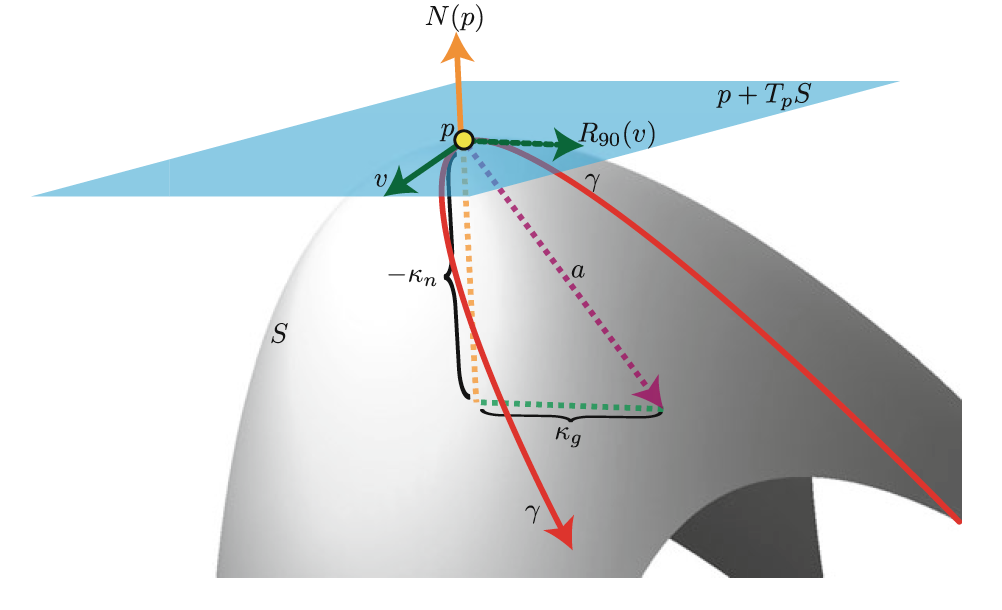
\includegraphics[width=12cm]{./images/normal_and_geodesic_curvature}
    \caption{The normal and geodesic curvature of \(\gamma\) at \(p\)}
    \label{fig:normal_and_geodesic_curvature}
\end{figure}


\end{document}